% !TEX program = lualatex
% !TEX encoding = UTF-8 Unicode
% 
\newcommand{\titol}{Sistemas basados en el conocimiento}
\newcommand{\materia}{Inteligencia artificial}
\newcommand{\idioma}{english,spanish}
\newcommand{\pdfauthors}{Nil Mamano Grande, Héctor Ramón Jiménez, Isaac Sánchez Barrera}
%\newcommand{\autors}[1]{\begin{tabular}{#1} Nil Mamano Grande \\ Héctor Ramón Jiménez \\ Isaac Sánchez Barrera\end{tabular}}
\newcommand{\autors}[1]{\begin{tabular}{#1} Mamano -- Ramón -- Sánchez\end{tabular}}
\newcommand{\data}{\today}
% !TEX encoding = UTF-8 Unicode
% !TEX root = report.tex
% 
\documentclass[a4paper,10pt,twoside,titlepage,abstract,numbers=noenddot,automark,mnsy,intlimits,rgb,dvipsnames]{scrartcl}
%\usepackage[utf8]{inputenc}
\usepackage{csquotes}
\usepackage[\idioma, es-tabla]{babel}
\spanishdecimal{.}
\usepackage{fontspec}
\defaultfontfeatures{Scale=MatchLowercase, Ligatures=TeX}
\usepackage{pdfpages}
\usepackage{fancyvrb}
\usepackage{amssymb}
\usepackage{amsmath}
\usepackage{mathtools}
\usepackage{unicode-math}
\unimathsetup{math-style=ISO,vargreek-shape=unicode}
\usepackage{xunicode}
\usepackage{ifxetex}
\usepackage{algorithm}
\usepackage{algpseudocode}

\ifxetex
  \usepackage{xltxtra}
\fi
\usepackage{verbatim}

\usepackage[binary-units]{siunitx}
\sisetup{
  product-units=single,
  list-units=single,
  per-mode=symbol,
  list-final-separator = { y },
  list-pair-separator = { y },
  range-phrase = { a },
}

\usepackage{fullpage}
\usepackage{framed}
\usepackage{xfrac}

\defaultfontfeatures{Path=fonts/, Scale=MatchLowercase}
\setmainfont[Ligatures=TeX,
BoldFont=texgyrepagella-bold.otf,
BoldItalicFont=texgyrepagella-bolditalic.otf,
ItalicFont=texgyrepagella-italic.otf]{texgyrepagella-regular.otf} %use this font
\setsansfont[Ligatures=TeX,
BoldFont=lmsans10-bold.otf,
BoldItalicFont=lmsans10-boldoblique.otf,
ItalicFont=lmsans10-oblique.otf]{lmsans10-regular.otf}
\setmonofont[BoldFont=lmmonolt10-bold.otf,
BoldItalicFont=lmmonolt10-boldoblique.otf,
ItalicFont=lmmono10-italic.otf,
SlantedFont=lmmonoslant10-regular.otf]{lmmono10-regular.otf}
\setmathfont{texgyrepagella-math.otf}
\setmathfont[range={\mathcal,\mathbfcal},StylisticSet=1]{xits-math.otf}

\usepackage[super]{nth}
%\setmathfont[ Path=fonts/, ]{LM Math}
%\usepackage{natbib}
\usepackage[natbib=true,language=english,style=numeric,citestyle=numeric,bibstyle=numeric,hyperref=true]{biblatex}

\usepackage{url}
\usepackage{pdflscape}
\usepackage{enumitem}

\usepackage{graphicx}
\usepackage{float}
\usepackage{caption}
\usepackage{subcaption}
\usepackage{multicol}
\usepackage{booktabs}

\usepackage[hidelinks]{hyperref}
\hypersetup{
    pdfencoding=auto,
    pdffitwindow=false,      % page fit to window when opened
    pdftitle={\materia\ :: \titol},    % title
    pdfauthor={\pdfauthors},     % author
    pdfsubject={},   % subject of the document
    pdfcreator={XeLaTeX + Hyperref package},
    colorlinks=false
}

\usepackage{setspace}

\usepackage[nouppercase]{scrpage2}

\setlength{\headheight}{15pt}
\renewcommand{\headfont}{\upshape}
\defpagestyle{curr}
  {    %% superior
    (\textwidth,0pt) %líneas
    {    %%par
      {\autors{l}}
      {\hfill}
      {\leftmark}
    }
    {	%%impar
      {\rightmark}
      {\hfill}
      {\autors{r}}
    }
    {	%% una sola cara
      {\thepart}
      {\hfill}
      {\autors{r}}
    }
    (\textwidth,0.5pt) %líneas
  }
  {		%% inferior
    (\textwidth,0.5pt) %líneas
    {	%%par
      {\thepage}
      {\hfill}
      {\materia}
    }
    {	%%impar
      {\titol}
      {\hfill}
      {\thepage}
    }
    {	%% una sola cara
      {\materia: \titol}
      {\hfill}
      {\thepage}
    }
    (\textwidth,0pt) %líneas
  }

\pagestyle{curr}

\headsep = 15pt
%\addtolength{\footskip}{-16pt}
%\addtolength{\textheight}{+16pt}
\addtolength{\topmargin}{-15pt}
\addtolength{\hoffset}{12mm}
\addtolength{\textwidth}{-11mm}
\usepackage{wrapfig}

\usepackage{amsthm}
%~ \theoremprework {\textcolor{white} {\rule{0.2in}{0.11in}} \hrule\rule{0.2in}{0.11in}}
%~ \theorempostwork {\hrule %\textcolor{white} {\rule{0.2in}{0.11in}}
%~ }

\makeatletter
\newcommand{\strong}[1]{\@strong{#1}}
\newcommand{\@@strong}[1]{\textbf{\let\@strong\@@@strong#1}}
\newcommand{\@@@strong}[1]{\textnormal{\let\@strong\@@strong#1}}
\let\@strong\@@strong
\makeatother

%~ \theoremindent0.5cm
%~ \theoremstyle{break}
%~ \theorembodyfont{}
%~ \newtheorem*{defi}{}

\theoremstyle{plain}% default
\newtheorem{thm}{Teorema}[section]
\newtheorem{lem}[thm]{Lemma}
\newtheorem{prop}{Proposition}
\newtheorem{cor}{Corollary}

\theoremstyle{definition}
\newtheorem{defn}{Definition}[section]
\newtheorem{conj}{Conjecture}[section]
\newtheorem{exmp}{Example}[section]

\theoremstyle{remark}
\newtheorem*{obs}{Observation}
\newtheorem*{note}{Remark}
\newtheorem{case}{Case}
\newtheorem*{notation}{Notation}

\addtolength{\voffset}{-15pt}
\addtolength{\headsep}{10pt}
\addtolength{\textheight}{35pt}
\addtolength{\footskip}{-20pt}
\addtolength{\textwidth}{15pt}
\addtolength{\marginparwidth}{-20pt}
\addtolength{\oddsidemargin}{-20pt}
\addtolength{\evensidemargin}{-20pt}

\usepackage{listings}

\definecolor{FonsCodi}{cmyk}{0,0,0,0.04}
\definecolor{Comentaris}{cmyk}{0,0,0,0.6}
\definecolor{mygreen}{rgb}{0,0.6,0}
\definecolor{mygray}{rgb}{0.6,0.6,0.6}
\definecolor{mymauve}{rgb}{0.58,0,0.82}
\definecolor{darkgreen}{rgb}{0.2,0.5,0.2}
\definecolor{orange}{rgb}{1,0.5,0}

\lstset{ %
language=Java,                % choose the language of the code
basicstyle=\ttfamily\small,
numbers=none,                   % where to put the line-numbers
numberstyle=\footnotesize,      % the size of the fonts that are used for the line-numbers
stepnumber=1,                   % the step between two line-numbers. If it's 1 each line will be numbered
numbersep=5pt,                  % how far the line-numbers are from the code
backgroundcolor=\color{FonsCodi},  % choose the background color. You must add \usepackage{color}
rulesepcolor=\color{FonsCodi},
lineskip=-2.5pt,
showspaces=false,               % show spaces adding particular underscores
showstringspaces=false,         % underline spaces within strings
showtabs=false,                 % show tabs within strings adding particular underscores
frame=single,                    % adds a frame around the code
tabsize=8,	                % sets default tabsize to 2 spaces
commentstyle=\itshape\color{Comentaris},
captionpos=t,                   % sets the caption-position to top
breaklines=true,                % sets automatic line breaking
breakatwhitespace=false,        % sets if automatic breaks should only happen at whitespace
escapeinside={\%*}{*)},          % if you want to add a comment within your code
keywordstyle=\bfseries\color{blue},
commentstyle=\itshape\color{darkgreen},
stringstyle=\color{orange},
}

\renewcommand{\lstlistlistingname}{Índice de códigos fuente}
\renewcommand{\lstlistingname}{Código fuente}

\setstretch{1.0}
\DefineBibliographyStrings{spanish}{%
  references = {Referencias},
}

\title{\materia\\
\Large{\titol}}
\subtitle{Facultat d'Informàtica de Barcelona\\ % Pongo la I mayúscula porque la FIB lo hace
Universitat Politècnica de Catalunya}
\author{
  Nil Mamano Grande \\
  Héctor Ramón Jiménez \\
  Isaac Sánchez Barrera}
\date{
  \today \\
  cuatrimestre de otoño \\
  curso 2013--2014}

\everymath{\displaystyle}

\newcommand{\CC}{\mathbb{C}}
\newcommand{\RR}{\mathbb{R}}
\newcommand{\NN}{\mathbb{N}}
\newcommand{\bigO}[1]{\ensuremath{\operatorname{O}\left(#1\right)}}% big-O notation/symbol
\newcommand{\bigOmega}[1]{\ensuremath{\operatorname{\Omega}\left(#1\right)}}% big-O notation/symbol
\newcommand{\bigTheta}[1]{\ensuremath{\operatorname{\Theta}\left(#1\right)}}% big-O notation/symbol
\newcommand{\slot}[1]{\texttt{\emph{#1}}}
\newcommand{\clase}[1]{\texttt{#1}}

\newenvironment{slotlist}{%
   \renewcommand\descriptionlabel[1]{\hspace{\labelsep}\slot{##1}}
   \begin{description}%
}{%
   \end{description}%
}

\bibliography{references}
\begin{document}

\maketitle
\tableofcontents
\listoftables
\listoffigures
\vfill
\cleardoublepage

\part{Presentación y análisis del problema}
% !TEX encoding = UTF-8 Unicode
% !TEX root = ../report.tex
% 

\begin{wrapfigure}{O}{0.3\textwidth}
  \vspace{-20pt}
  \begin{center}
    
\includegraphics[width=0.28\textwidth]{figures/ricorico}
  \end{center}
  \vspace{-20pt}
\end{wrapfigure}

\section{Introducción}
\subsection{Descripción del problema}
La empresa de catering \emph{Rico Rico} quiere mejorar su eficiencia a la hora
de proponer menús para las celebraciones de sus clientes. Con ese fin, ha
encargado la implementación de un sistema experto basado en el conocimiento que
tienen tras su larga experiencia en el sector. Gracias al sistema, solamente es
necesario que el cliente indique sus preferencias y restricciones concretas
para obtener las recomendaciones más acordes con sus necesidades.



% !TEX encoding = UTF-8 Unicode
% !TEX root = ../report.tex
% 

\section{Conceptualización del problema}
\subsection{Conceptos principales del dominio}

Después de haber hecho un trabajo iterativo, los conceptos que se modelan en el
dominio de conocimiento son
\begin{enumerate}
  \item Cosas elaboradas, como platos y vino (tienen su nombre y precio).
  \item Dentro de los platos, si son pesados o ligeros y su dificultad de
    preparación.
  \item Los ingredientes que forman parte de los platos y su disponibilidad
    durante las cuatro estaciones del año.
  \item Grandes grupos de comensales, que modelan el tipo de ingredientes que
    no pueden comer.
  \item Los tipos de platos, que contienen información sobre los vinos que
    pueden ir mejor con ellos.
  \item Los eventos a celebrar, que tienen los platos que son propios (o
    recomendables) y la importancia de éstos últimos a la hora de elaborar el
    los menús para el cliente.
  \item Las regiones de procedencia de los platos.
  \item El estilo de los platos. Están los genéricos, que no llegarían a ser
    tradicionales porque son simples platos, los tradicionales (podrían
    considerarse, en parte, folclóricos), y platos modernos. Además, también se
    hace distinción de los platos para sibaritas, que son para los paladares
    más finos, pero que pueden pertenecer a cualquiera de las categorías
    anteriores.
\end{enumerate}

Como hemos indicado anteriormente, los comensales que no beben vino acostumbran
a preferir una bebida concreta de forma individualizada. Por esta razón, hemos
pensado que no es algo a modelar en nuestro dominio de conocimiento.

Por otro lado, en el dominio de solución disponemos de
\begin{enumerate}
  \item Recomendaciones concretas de platos, con los motivos para su
    recomendación y una valoración.
  \item Posibles menús abstractos, que contienen el orden de platos y los
    colores de los vinos más aptos para éstos.
  \item Los menús finales con los platos y vinos concretos, además de las
    razones y valoración de su recomendación.
\end{enumerate}

\vfill
\clearpage
\part{Implementación del sistema experto}
% !TEX encoding = UTF-8 Unicode
% !TEX root = ../report.tex
% 

\section{Construcción de la ontología}

\begin{figure}[h!]
  \makebox[\textwidth][c]{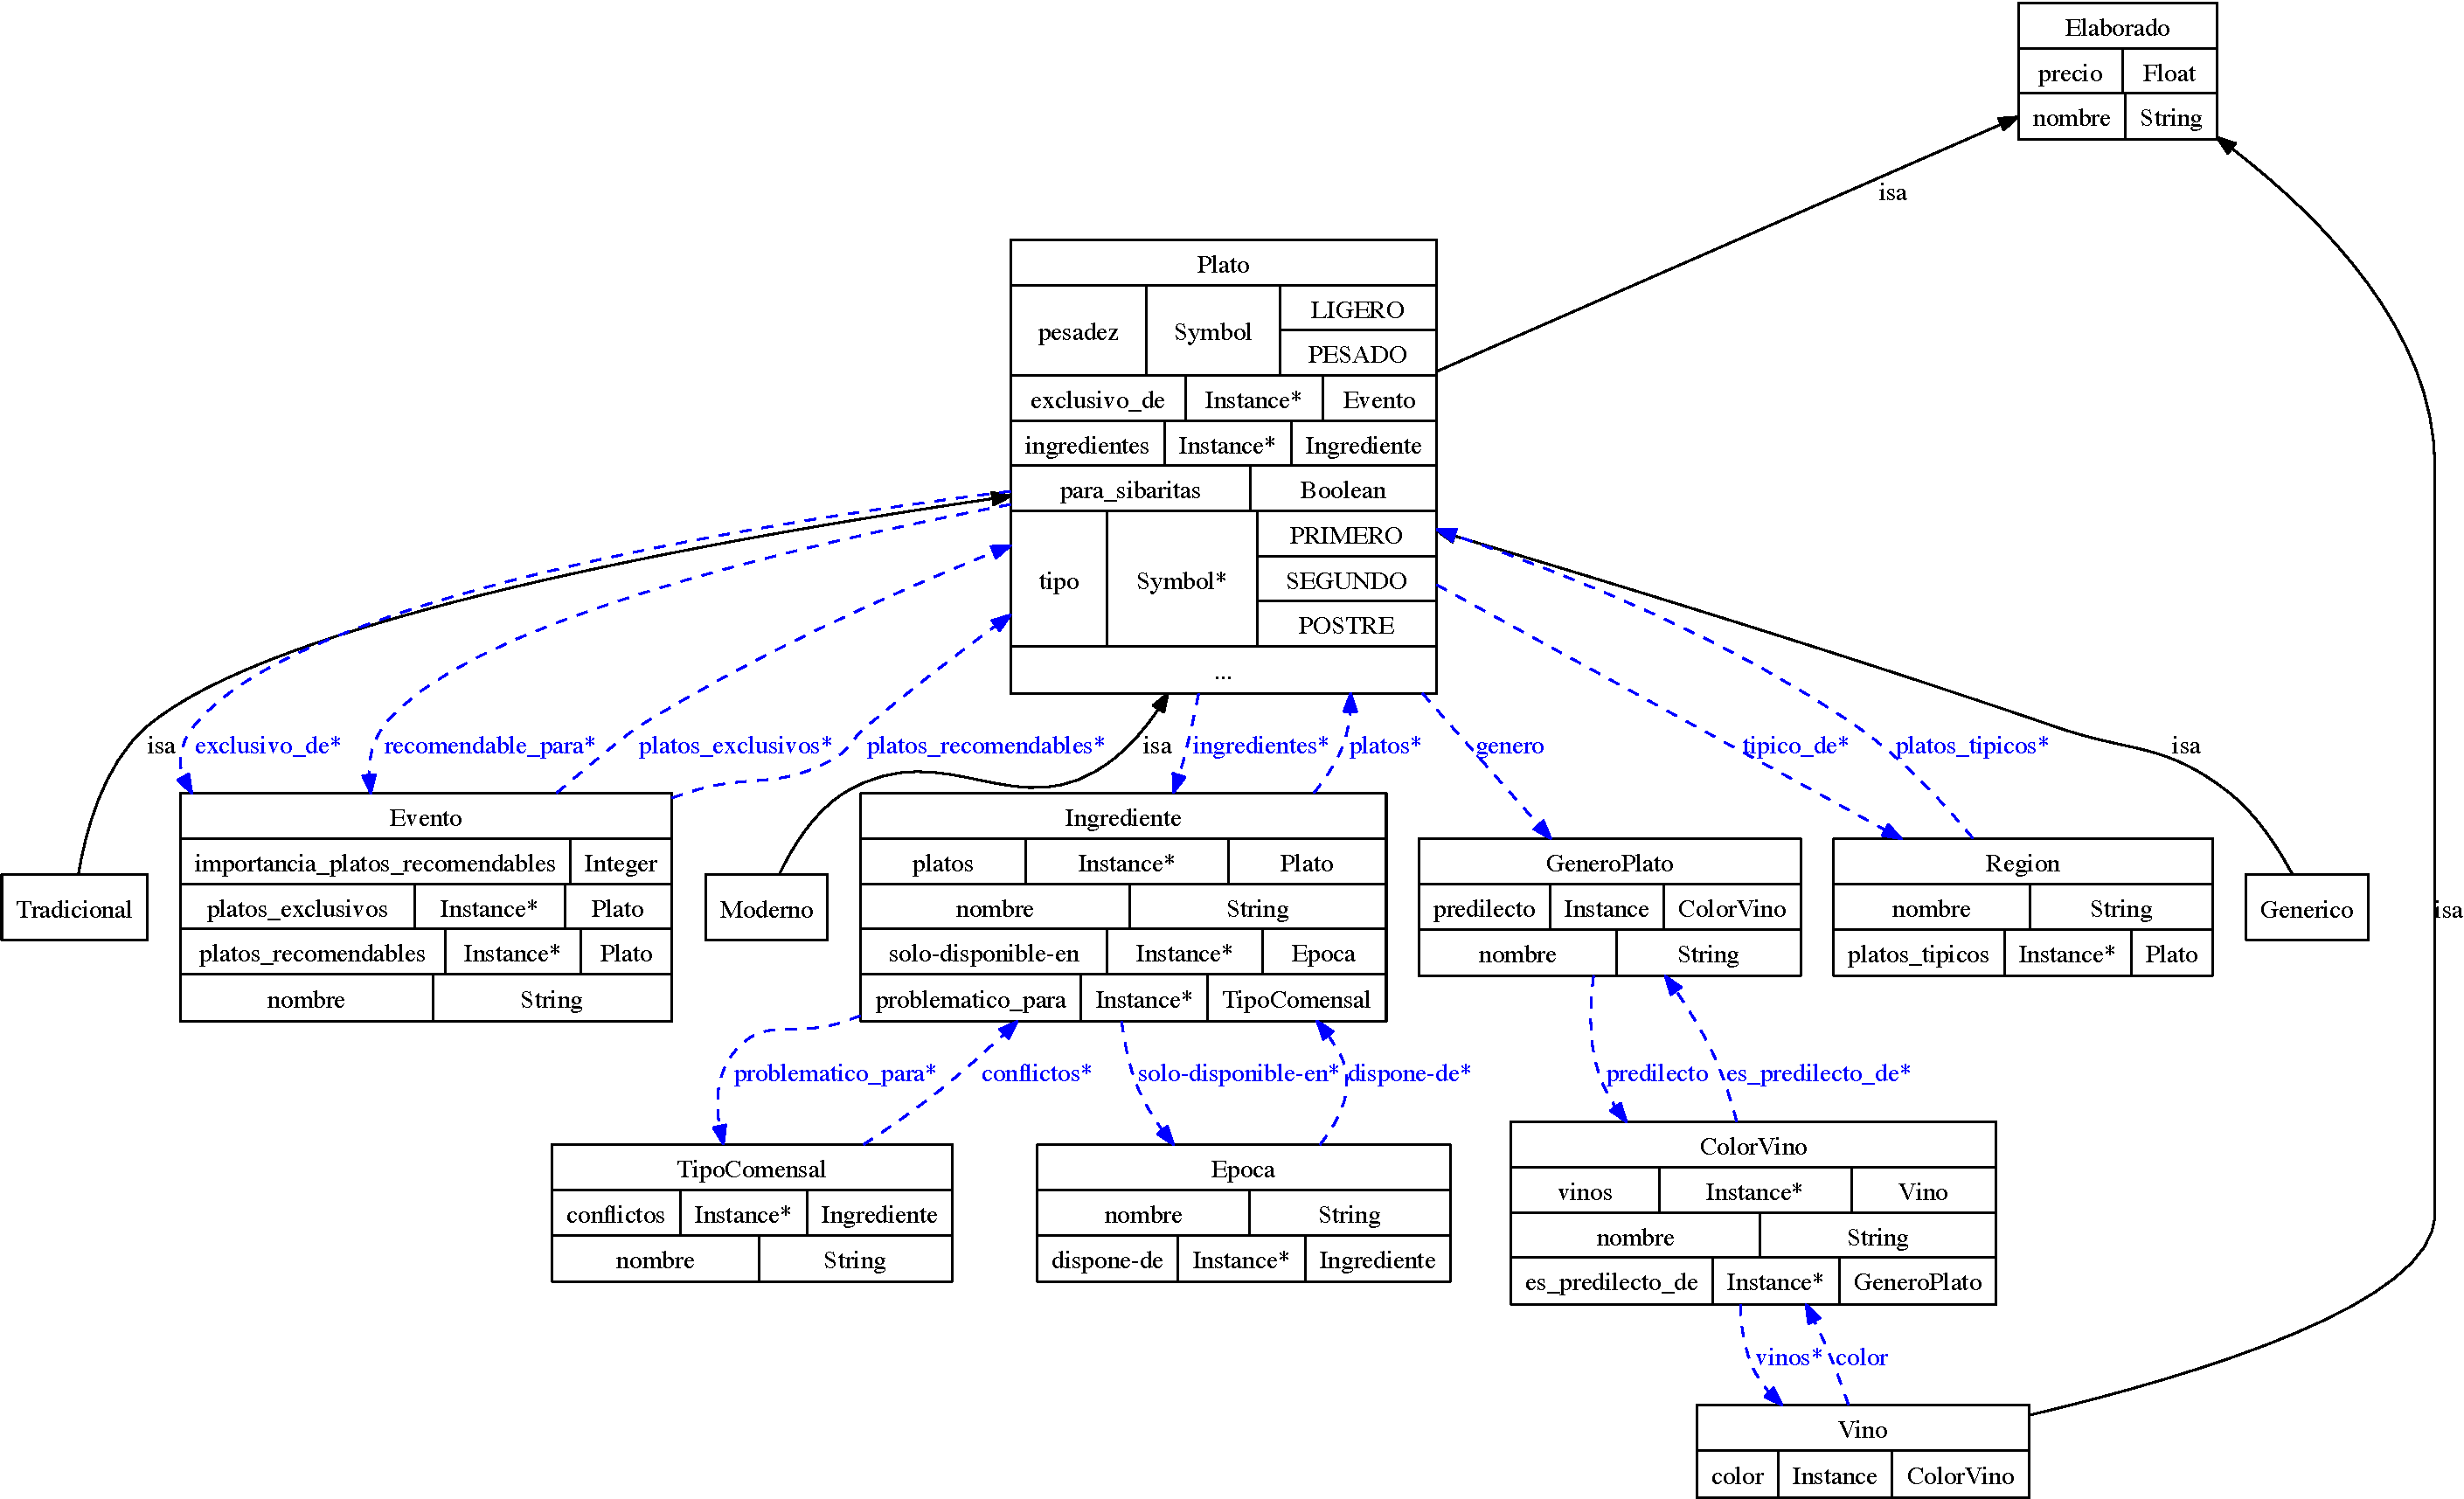
\includegraphics[width=1.2\textwidth]{%
      figures/ontologia}}
  \caption{La ontología final}
\end{figure}

La construcción de la ontología (y de todo el sistema en general) se ha
realizado de manera iterativa, aunque inicialmente no había sido así.

En un principio habíamos construido sistema de clases completo pero incluso más
complejo de lo que ha sido finalmente, sin necesidad. Afortunadamente, esa
versión se perdió y empezamos con una más simple que solamente contenía las
clases elaborado, plato, bebida (que ahora es solamente vino) e ingrediente.

Luego añadimos la clase de tipos de comensal, para poder tener en cuenta
alergias y demás problemas alimenticios. También se añadió la clase época para
poder indicar la disponibilidad de ingredientes.

Inicialmente, los eventos iban a ser unos valores prefijados hasta que vimos
que podríamos sacarle más provecho a todo si eran instancias dentro de la
ontología. Así que creamos la clase evento y asociamos algunos platos como
preferidos en el evento. Para evitar que determinados platos propios de un
evento se recomendaran en otros donde no tuviera sentido (un claro ejemplo son
los pasteles de boda), casi al final hicimos la diferencia entre platos propios
y platos que son recomendables para los eventos.

Ya, más entrados en el proceso de implementación del sistema experto, añadimos
la clase región para poder modelar el origen geográfico/cultural de los
platos. Finalmente, cuando empezamos a tratar con los vinos, y tras considerar
que la bebida en general no tiene sentido para el problema que se nos pide
resolver, eliminamos la clase bebida, dejando solamente una clase para
vinos. Además, creamos la clase que modela el color del vino, que se asoció a
la nueva clase de géneros de plato (sopa, pescado, estofado, aperitivo, etc.)
para poder hacer la recomendación de vinos de manera más sencilla.

Fuera de aquí, también están las ontologías de solución del problema, que
solamente contienen las clases menú y menú abstracto. Más adelante detallaremos
su funcionamiento.

\subsection{Detalle de las clases de la ontología del problema}
\subsubsection{Clase \texttt{Elaborado}}
Esta clase está construida para agrupar las características propias de los
productos que se venden con el menú: el \slot{nombre} y el
\slot{precio}. La idea es que cualquier cosa que esté en el menú debe ser un
producto elaborado.

En determinado momento tuvimos que hacer esta clase concreta para poder hacer
\emph{pattern matching} con CLIPS. Por suerte, los cambios que fuimos haciendo
en la implementación del problema provocaron que esta clase pudiera volver a
ser abstracta. Mientras la clase fue concreta, la clase \verb+Plato+ también
tuvo que serlo porque CLIPS no permite subclases abstractas de clases
concretas.

\subsubsection{Clase \texttt{Plato} y sus subclases}
La clase es abstracta y está dividida en las subclases \verb+Generico+,
\verb+Moderno+ y \verb+Tradicional+. Hemos decidido hacer esta clasificación
porque no es habitual que un plato sea moderno y tradicional a la vez, y
también existen platos que no se considerarían tradicionales pero que son
platos que se consumen habitualmente (de ahí el término genérico).

Además del nombre y el precio derivados de \verb+Elaborado+, la clase
\verb+Plato+ proporciona nuevos campos:
\begin{slotlist}
\item[ingredientes] Es un campo múltiple de instancias de la clase
  \verb+Ingrediente+. Es necesario que haya como mínimo un ingrediente.
\item[genero] Es un campo simple que apunta a una instancia de
  \verb+GeneroPlato+. Sirve para clasificar los platos en sus géneros.
\item[tipo] Un campo múltiple que indica si el plato es \emph{primero},
  \emph{segundo} o \emph{postre}. Es necesario que sea algún tipo de plato.
\item[para\_sibaritas] Un campo cierto/falso. Los platos para sibaritas no
  queremos que se recomienden a alguien que no lo es, pues es habitual que no
  lo quieran. Por otro lado, se les da prioridad si el cliente sí lo es.
\item[temperatura] Indica si el plato es frío o caliente.
\item[pesadez] Indica si un plato es ligero o pesado. En general, no es bueno
  que un cliente coma dos platos ligeros o dos platos pesados.
\item[tipico\_de] Es un campo múltiple que contiene las instancias de
  \verb+Region+ de donde es típico el plato, si es el caso.
\item[recomendable\_para] Un campo múltiple que contiene, si es el caso, en qué
  eventos pueden preferir el plato, para que se priorice.
\item[exclusivo\_de] A diferencia del anterior, si está definido indica en qué
  eventos puede ofrecerse el plato de forma exclusiva (por ejemplo, un pastel
  de boda solamente puede ofrecerse en una boda). También lo prioriza.
\item[dificultad] Indica, mediante un valor de 0 a 100, la dificultad de
  elaboración del plato (un valor mayor indica una dificultad mayor). Cuantos
  más comensales hay en la celebración, más importante es que el plato sea más
  sencillo de elaborar.
\end{slotlist}

Las subclases de \verb+Plato+ no contienen ningún slot propio. Simplemente es
para poder separar correctamente y poder hacer uso del \emph{pattern matching}
en CLIPS.

\subsubsection{Clase \texttt{GeneroPlato}}
Mediante esta clase se modelan los distintos géneros de plato en función de
cómo son. Es decir, sopas, platos de pescado, estofados, etc. Se utiliza para
poder agrupar platos similares que precisan vinos de colores similares. Por
tanto, además del \slot{nombre} del género, el único campo que tienen es
\slot{predilecto}, que apunta al color de vino más acorde con los platos de ese
género.

No tienen el campo inverso hacia \verb+Plato+ con los platos del género porque
no lo usamos durante el problema.

\subsubsection{Clase \texttt{Vino}}
Esta clase representa a los vinos. Además de los campos de \verb+Elaborado+,
contiene un campo \slot{color} que apunta a la instancia de \verb+ColorVino+
con el color del vino.

\subsubsection{Clase \texttt{ColorVino}}
Como ya hemos comentado con anterioridad, esta clase representa los colores que
puede tomar un vino. Los campos que tiene, además del \slot{nombre} del color, son dos:
\begin{slotlist}
\item[es\_predilecto\_de] Es el campo múltiple que contiene la lista de géneros
  de plato que prefieren ese color de vino. Por tanto, es el inverso del campo
  \verb+ColorVino+:\slot{predilecto}.
\item[vinos] Este campo múltiple guarda la lista de vinos del color. Es el campo inverso a \verb+Vino+:\slot{color}.
\end{slotlist}

\end{document}
